\documentclass[titlepage, parkskip=full, twocolumn, landscape]{scrartcl}
\usepackage[ngerman]{babel}
\usepackage[T1]{fontenc}
\usepackage[utf8]{inputenc}

\usepackage{amsmath}
\usepackage{graphicx}
\usepackage[hidelinks]{hyperref}

\title{Physik}
\author{Die \textsc{Wikipedia}-Autoren\thanks{Dies ist eine Kopie des Artikels \url{https://de.wikipedia.org/wiki/Physik}, Stand 8.\,10.\,2017. Es wurde lediglich die Schrödingergleichung auf Seite~\pageref{eq:schrödinger} eingefügt, um den Formelsatz zu demonstrieren.}}
\date{8.\,10.~2017}
\titlehead{"To be honest you really need to have a solid grasp on theoretical Physics to get Rick and Morty"}
\subject{Die neue germanische}
\subtitle{Die Rückkehr}
\publishers{Albert Einstein}
\begin{document}

\maketitle

\tableofcontents

\begin{figure}
	\centering
	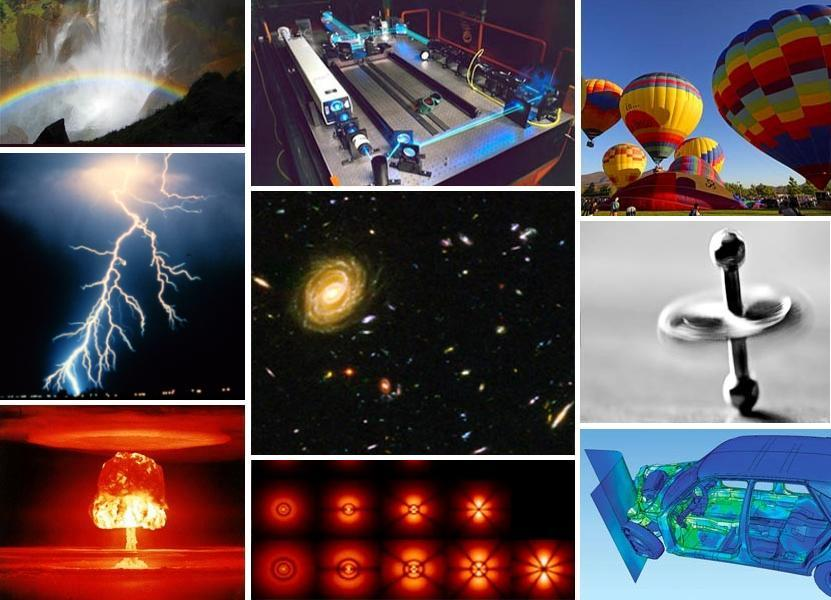
\includegraphics[width=12cm]{images/1.jpg}
	\caption{Verschiedene Beispiele physikalischer Phänomene}
\end{figure}

\noindent Die \textbf{Physik} (über lateinisch \emph{physica} "`Naturlehre"')\footnote{Wilhelm Gemoll: \emph{Griechisch-Deutsches Schul- und Handwörterbuch.} München/Wien 1965.} \footnote{Erich Pertsch: \emph{Langenscheidts Großes Schulwörterbuch Lateinisch-Deutsch.} Langenscheidt, Berlin 1978, ISBN 3-468-07201-5} ist eine Naturwissenschaft und untersucht die grundlegenden Phänomene in der Natur. Um deren Eigenschaften und Verhalten anhand von quantitativen Modellen und Gesetzmäßigkeiten zu erklären, befasst sie sich insbesondere mit Materie und Energie und deren Wechselwirkungen in Raum und Zeit.

Erklären bedeutet hier einordnen, vergleichen, allgemeineren Erscheinungen zuordnen oder aus allgemeiner gültigen Naturgesetzen folgern.\footnote{Richard Feynman schrieb dazu: \emph{Die Neugier verlangt, dass wir fragen, dass wir \dots{} versuchen, die Vielfalt der Gesichtspunkte vielleicht als Ergebnis des Zusammenwirkens einer relativ geringen Anzahl elementarer Dinge und Kräfte zu verstehen \dots} Richard P. Feynman u.\,a.: \emph{Feynman Vorlesungen über Physik}. Bd.~1, Teil~1, übersetzt von H.~Köhler. Deutsch-engl. Ausgabe, Oldenbourg Verlag 1974, Seite 2--1.} Dazu ist häufig die Bildung geeigneter neuer Begriffe nötig, teilweise auch solcher, die der unmittelbaren Anschauung nicht mehr zugänglich sind. Erklärungen in dem philosophischen Sinn, "`warum"' die Natur sich so und nicht anders verhält, kann die Physik nicht leisten.

Die Arbeitsweise der Physik besteht in einem Zusammenwirken experimenteller Methoden und theoretischer Modellbildung. Physikalische Theorien bewähren sich in der Anwendung auf Systeme der Natur, indem sie bei Kenntnis von deren Anfangszuständen Vorhersagen über spätere Zustände erlauben. Erkenntnisfortschritte ergeben sich durch das Wechselspiel von Beobachtung oder Experiment mit der Theorie. Eine neue oder weiterentwickelte Theorie kann bekannte Ergebnisse besser oder überhaupt erstmals erklären und darüber hinaus neue Experimente und Beobachtungen anregen, deren Ergebnisse dann die Theorie bestätigen oder ihr widersprechen. Unerwartete Beobachtungs- oder Versuchsergebnisse geben Anlass zur Theorieentwicklung in verschiedener Gestalt, von schrittweiser Verbesserung bis hin zur völligen Aufgabe einer lange Zeit akzeptierten Theorie.

Erkenntnisfortschritte führen beispielsweise zur Ausdehnung oder Einschränkung des Gültigkeitsbereichs einer Theorie, zu genaueren Beschreibungen, Vereinfachungen des theoretischen Apparats oder zu neuen oder erleichterten praktischen Anwendungen.
\begin{equation}
	\mathrm{i}\hbar\frac{\partial}{\partial t} \psi(\vec{r},t) = \left(-\frac{\hbar^2}{2m}\Delta + V(\vec{r},t)\right) \psi(\vec{r},t) \label{eq:schrödinger}
\end{equation}
Erkenntnisse und Modelle aus der Physik werden intensiv in der Chemie, Geologie, Biologie, Medizin und vielen Ingenieurwissenschaften genutzt, in neuerer Zeit auch in Zweigen der Sozialwissenschaften und Wirtschaftswissenschaften.

\section{Geschichte von Begriff und Disziplin der Physik}

Die Disziplin der Physik in ihrer heutigen Gestalt hat ihre Ursprünge in der Philosophie, die sich seit der Antike im weitesten Sinne mit den Gründen und Ursachen aller Dinge befasst. Von Aristoteles bis ins beginnende 19. Jahrhundert wurde die Physik als das Teilgebiet der Philosophie verstanden, das sich als \emph{Naturlehre, Naturgeschichte, Chemie} oder \emph{angewandte Mathematik} mit den Gegebenheiten der Natur beschäftigt.\footnote{Rudolf Stichweh: \emph{Zur Entstehung des modernen Systems wissenschaftlicher Disziplinen -- Physik in Deutschland 1740--1890}, Suhrkamp Verlag, Frankfurt 1984.} Gegenüber den rein philosophischen Erklärungsversuchen der Naturvorgänge spielte die Art von Erkenntnis, die durch systematische und genaue Beobachtung, also empirisch zu gewinnen ist, lange Zeit keine Rolle. Ab Mitte des 13. und im Laufe des 14. Jahrhunderts plädierten dann einzelne Philosophen und Naturforscher -- meist ein- und dieselbe Person wie etwa Roger Bacon -- für ein größeres Gewicht der durch Beobachtung zu erlangenden Naturerkenntnis. Diese Tendenzen mündeten im 16. und 17. Jahrhundert, namentlich mit Galileo Galilei und Isaac Newton, in die Entwicklung einer Methodologie der physikalischen Erkenntnis, die vorrangig an empirischen und sogar experimentellen Standards orientiert ist und diesen vor überkommenen philosophischen Grundsätzen im Zweifelsfall sogar den Vorrang einräumt. Dieser Ansatz wurde zunächst als "`experimentelle Philosophie"' bezeichnet und führte beim Verständnis vieler unterschiedlicher Naturvorgänge rasch zu bedeutendem Erfolgen. Dennoch dauerte es noch bis ins 19. Jahrhundert, dass er sich endgültig in der Physik durchsetzen konnte und sie damit als eigenständige Disziplin in ihrem heutigen Sinn etablierte.

Hinsichtlich ihrer Methode, ihres Gegenstandsbereichs, ihrer wissenschaftssystematischen und institutionellen Verortung teilt sich die Physik im Wesentlichen in zwei große Gebiete auf. Die theoretische Physik beschäftigt sich vorwiegend mit formalen mathematischen Beschreibungen und den Naturgesetzen. Sie abstrahiert Vorgänge und Erscheinungen in der wirklichen Natur in Form eines Systems von Modellen, allgemeingültigen Theorien und Naturgesetzen sowie intuitiv gewählten Hypothesen. Bei der Formulierung von Theorien und Gesetzen bedient sie sich vielfach der Methoden der Mathematik und der Logik. Ziel ist, das Verhalten eines Systems theoretisch vorherzusagen, damit dies durch Vergleich mit den Vorgängen und Erscheinungen in der wirklichen Natur überprüft werden kann. Diese Überprüfung in Form reproduzierbarer Messungen an gezielt gestalteten physikalischen Experimenten oder durch Beobachtung natürlicher Phänomene ist das Gebiet der Experimentalphysik. Das Ergebnis der Überprüfung bestimmt über die Gültigkeit und Vorhersagekraft des Modells und der darin gewählten Begriffe, Hypothesen und Methoden.

Die Physik steht in enger Verbindung zu den Ingenieurwissenschaften und den anderen Naturwissenschaften von der Astronomie und Chemie bis zur Biologie und den Geowissenschaften. Die Physik wird dabei häufig als grundlegende oder fundamentale Naturwissenschaft aufgefasst, die sich am stärksten mit den Grundprinzipien befasst, die die natürlichen Vorgänge bestimmen. Die Grenzziehung zu den anderen Naturwissenschaften hat sich historisch ergeben, wird jedoch insbesondere mit dem Aufkommen neuer Wissenschaftsdisziplinen immer schwieriger.

In der heutigen Physik ist vor allem die durch Atom- und Molekülphysik und Quantenchemie markierte Grenze zur Chemie fließend. Zur Abgrenzung gegenüber der Biologie wurde die Physik oftmals als die Wissenschaft von der unbelebten im Gegensatz zur belebten Natur bezeichnet, womit jedoch eine Beschränkung impliziert wird, die so in der Physik nicht existiert. Die Ingenieurwissenschaften sind durch ihren engen Bezug zur praktischen technischen Anwendung von der Physik abgegrenzt, da in der Physik das Verständnis der grundlegenden Mechanismen im Vordergrund steht. Die Astronomie hat keine Möglichkeit, Laborexperimente durchzuführen, und ist daher allein auf Naturbeobachtung angewiesen, was hier zur Abgrenzung gegen die Physik herangezogen wird.

\section{Methodik}

Die Erkenntnisgewinnung in der Physik verläuft in enger Verzahnung von Experiment und Theorie, besteht also aus empirischer Datengewinnung und -auswertung \emph{und} gleichzeitig dem Erstellen theoretischer Modelle zu ihrer Erklärung. Dennoch haben sich im Verlauf des 20. Jahrhunderts Spezialisierungen herausgebildet, die insbesondere die professionell betriebene Physik heute prägen. Demnach lassen sich grob Experimentalphysik und theoretische Physik voneinander unterscheiden.

\subsection{Experimentalphysik}

\begin{figure}
	\centering
	
\includegraphics[width=4cm]{images/2.jpg}
	\caption{Multimeter für elektrische Messungen}
\end{figure}

Während manche Naturwissenschaften wie etwa die Astronomie und die Meteorologie sich methodisch weitgehend auf Beobachtungen ihres Untersuchungsgegenstandes beschränken müssen, steht in der Physik das Experiment im Vordergrund. Die Experimentalphysik versucht durch Entwurf, Aufbau, Durchführung und Auswertung von Experimenten Gesetzmäßigkeiten aufzuspüren und mittels empirischer Modelle zu beschreiben. Sie versucht einerseits physikalisches Neuland zu betreten, andererseits überprüft sie von der theoretischen Physik gemachte Vorhersagen.

Grundlage eines physikalischen Experimentes ist es, die Eigenschaften eines zuvor präparierten physikalischen Systems, zum Beispiel eines geworfenen Steins, eines eingeschlossenen Gasvolumens oder eines Teilchens bei einem Stoßprozess durch Messung in Zahlenform auszudrücken, etwa als Aufprallgeschwindigkeit, als resultierender Druck (bei gegebenen Randbedingungen) oder als Länge der beobachtbaren Teilchenspuren im Detektor.

Konkret werden entweder nur die zeitunabhängigen (\emph{statischen}) Eigenschaften eines Objektes gemessen oder es wird die zeitliche Entwicklung (\emph{Dynamik}) des Systems untersucht, etwa indem Anfangs- und Endwerte einer Messgröße vor und nach dem Ablauf eines Vorgangs bestimmt werden oder indem kontinuierliche Zwischenwerte festgestellt werden.

\subsection{Theoretische Physik}

\begin{figure}
	\centering
	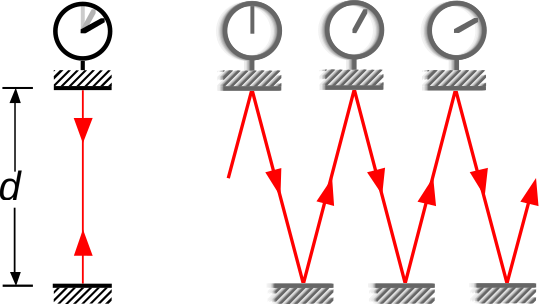
\includegraphics[width=5cm]{images/3}
	\caption{Die Lichtuhr, ein bekanntes Gedankenexperiment}
\end{figure}

Die theoretische Physik sucht die empirischen Modelle der Experimentalphysik mathematisch auf bekannte Grundlagentheorien zurückzuführen oder, falls dies nicht möglich ist, Hypothesen für eine neue Theorie zu entwickeln, die dann experimentell überprüft werden können. Sie leitet weiterhin aus bereits bekannten Theorien empirisch überprüfbare Voraussagen ab.

Bei der Entwicklung eines Modells wird grundsätzlich die Wirklichkeit idealisiert; man konzentriert sich zunächst nur auf ein vereinfachtes Bild, um dessen Aspekte zu überblicken und zu erforschen. Nachdem das Modell für diese Bedingungen ausgereift ist, wird es weiter verallgemeinert.

Zur theoretischen Beschreibung eines physikalischen Systems benutzt man die Sprache der Mathematik. Seine Bestandteile werden dazu durch mathematische Objekte wie zum Beispiel Skalare oder Vektoren repräsentiert, die in durch Gleichungen festgelegten Beziehungen zueinander stehen. Aus bekannten Größen werden unbekannte errechnet und damit zum Beispiel das Ergebnis einer experimentellen Messung vorhergesagt. Diese auf Quantitäten konzentrierte Sichtweise unterscheidet die Physik maßgeblich von der Philosophie und hat zur Folge, dass nicht quantifizierbare Modelle, wie das Bewusstsein, nicht als Teil der Physik betrachtet werden.

Das fundamentale Maß für den Erfolg einer naturwissenschaftlichen Theorie ist die Übereinstimmung mit Beobachtungen und Experimenten. Durch den Vergleich mit dem Experiment lassen sich der Gültigkeitsbereich und die Genauigkeit einer Theorie ermitteln; allerdings lässt sie sich niemals "`beweisen"'. Um eine Theorie zu widerlegen oder die Grenzen ihres Gültigkeitsbereiches zu zeigen, genügt im Prinzip ein einziges Experiment, sofern es sich als reproduzierbar erweist.

Experimentalphysik und theoretische Physik stehen also in steter Wechselbeziehung zueinander. Es kann allerdings vorkommen, dass Ergebnisse der einen Disziplin der anderen vorauseilen: So sind derzeit viele Voraussagen der Stringtheorie nicht experimentell überprüfbar; andererseits sind viele teilweise sehr genau gemessene Werte aus dem Gebiet der Teilchenphysik zum heutigen Zeitpunkt (2009) durch die zugehörige Theorie, die Quantenchromodynamik, nicht berechenbar.

\subsection{Weitere Aspekte}

Zusätzlich zu dieser grundlegenden Teilung der Physik unterscheidet man manchmal noch weitere methodische Unterdisziplinen, vor allem die mathematische Physik und die angewandte Physik. Auch die Arbeit mit Computersimulationen hat Züge eines eigenen Bereiches der Physik.

\subsubsection{Mathematische Physik}

Die mathematische Physik wird gelegentlich als Teilgebiet der theoretischen Physik betrachtet, unterscheidet sich von dieser jedoch darin, dass ihr Studienobjekt nicht konkrete physikalische Phänomene sind, sondern die Ergebnisse der theoretischen Physik selbst. Sie abstrahiert damit von jedweder Anwendung und interessiert sich stattdessen für die \emph{mathematischen} Eigenschaften eines Modells, insbesondere seine tiefer liegenden Symmetrien. Auf diese Weise entwickelt sie Verallgemeinerungen und neue mathematische Formulierungen bereits bekannter Theorien, die dann wiederum als Arbeitsmaterial der theoretischen Physiker in der Modellierung empirischer Vorgänge Einsatz finden können.

\subsubsection{Angewandte Physik}

Die angewandte Physik steht in (unscharfer) Abgrenzung zur Experimentalphysik, teilweise auch zur theoretischen Physik. Ihr wesentliches Kennzeichen ist, dass sie ein gegebenes physikalisches Phänomen nicht um seiner selbst willen erforscht, sondern um die aus der Untersuchung hervorgegangenen Erkenntnisse zur Lösung eines (in der Regel) nicht-physikalischen Problems einzusetzen. Ihre Anwendungen liegen auf dem Gebiet der Technik oder Elektronik aber auch in den Wirtschaftswissenschaften, wo im Risikomanagement Methoden der theoretischen Festkörperphysik zum Einsatz kommen. Auch gibt es die interdisziplinären Bereiche der Medizinphysik, physikalischen Chemie, Astrophysik und Biophysik.

\subsubsection{Simulation und Computerphysik}

Mit der fortschreitenden Entwicklung der Rechensysteme hat sich in den letzten Jahrzehnten des 20. Jahrhunderts, beschleunigt seit etwa 1990, die Computersimulation als neue Methodik innerhalb der Physik entwickelt. Computersimulationen werden häufig als Bindeglied zwischen Theorie und Experiment verwendet, um Vorhersagen aus einer Theorie zu gewinnen, andererseits können Simulationen auch in Form einer effektiven Theorie, die ein experimentelles Ergebnis nachmodelliert, einen Impuls an die theoretische Physik zurückgeben. Naturgemäß hat dieser Bereich der Physik zahlreiche Anknüpfungspunkte an die Informatik.

\section{Theoriengebäude}

Das Theoriengebäude der Physik beruht in seinem Ursprung auf der klassischen Mechanik. Diese wurde im 19. Jahrhundert um weitere Theorien ergänzt, insbesondere den Elektromagnetismus und die Thermodynamik. Die moderne Physik beruht auf zwei Erweiterungen aus dem 20. Jahrhundert, der Relativitätstheorie und der Quantenphysik, die bestimmte Grundprinzipien der klassischen Mechanik verallgemeinert haben. Beide Theorien enthalten die klassische Mechanik über das sogenannte Korrespondenzprinzip als Grenzfall und haben daher einen größeren Gültigkeitsbereich als diese. Während die Relativitätstheorie teilweise auf denselben konzeptionellen Grundlagen beruht wie die klassische Mechanik, löst sich die Quantenphysik deutlich davon.

\subsection{Klassische Mechanik}

\begin{figure}
	\centering
	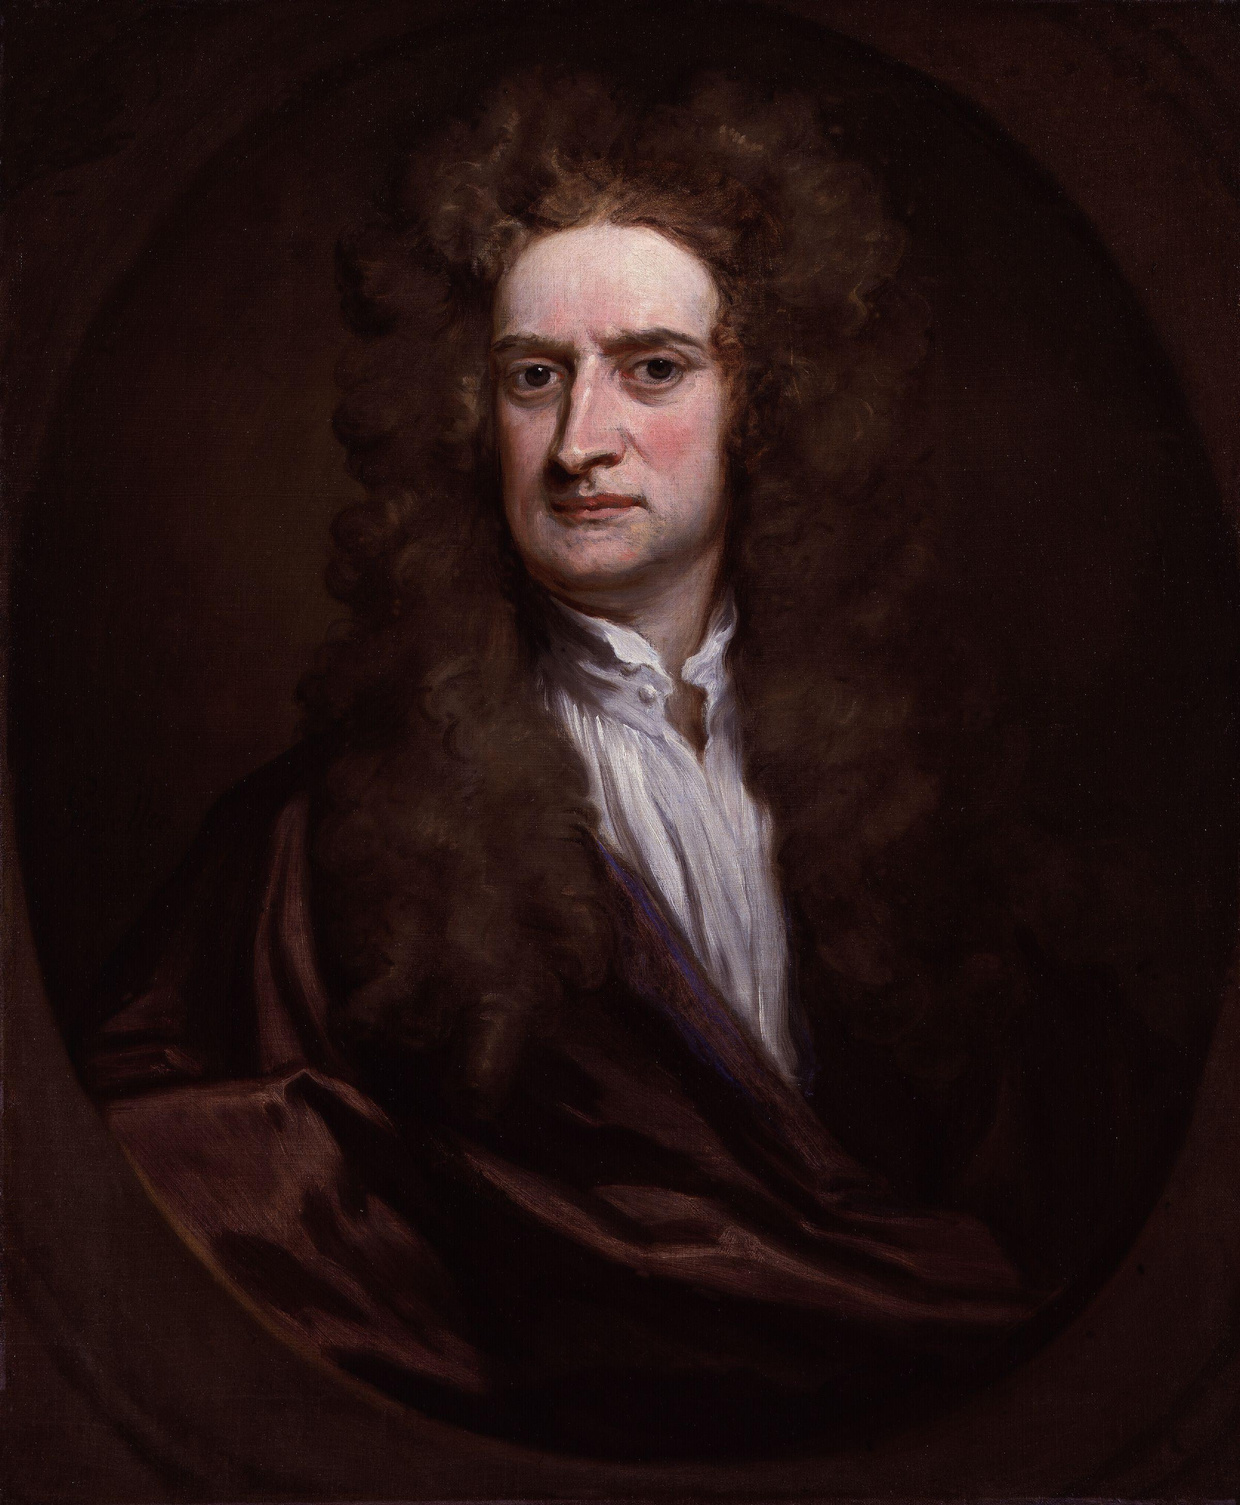
\includegraphics[width=5cm]{images/4.jpg}
	\caption{Isaac Newton}
\end{figure}

Die klassische Mechanik wurde im 16. und 17. Jahrhundert maßgeblich von Galileo Galilei und Isaac Newton begründet. Aufgrund der zu dieser Zeit noch recht begrenzten technischen Möglichkeiten sind die Vorgänge, die die klassische Mechanik beschreibt, weitgehend ohne komplizierte Hilfsmittel beobachtbar, was sie anschaulich erscheinen lässt. Die klassische Mechanik behandelt Systeme mit wenigen massiven Körpern, was sie von der Elektrodynamik und der Thermodynamik unterscheidet. Raum und Zeit sind dabei nicht Teil der Dynamik, sondern ein unbewegter Hintergrund, vor dem physikalische Prozesse ablaufen und Körper sich bewegen. Für sehr kleine Objekte tritt die Quantenphysik an die Stelle der klassischen Mechanik, während die Relativitätstheorie zur Beschreibung von Körpern mit sehr großen Massen und Energien geeignet ist.

Die mathematische Behandlung der klassischen Mechanik wurde im späten 18. und frühen 19. Jahrhundert in Form des Lagrange-Formalismus und des Hamilton-Formalismus entscheidend vereinheitlicht. Diese Formalismen sind auch mit der Relativitätstheorie anwendbar und sind daher ein bedeutender Teil der klassischen Mechanik. Obwohl die klassische Mechanik nur für mittelgroße, anschauliche Systeme gültig ist, ist die mathematische Behandlung komplexer Systeme bereits im Rahmen dieser Theorie mathematisch sehr anspruchsvoll. Die Chaostheorie befasst sich in großen Teilen mit solchen komplexen Systemen der klassischen Mechanik und ist derzeit (2009) ein aktives Forschungsgebiet.

\subsection{Elektrodynamik}

\begin{figure}
	\centering
	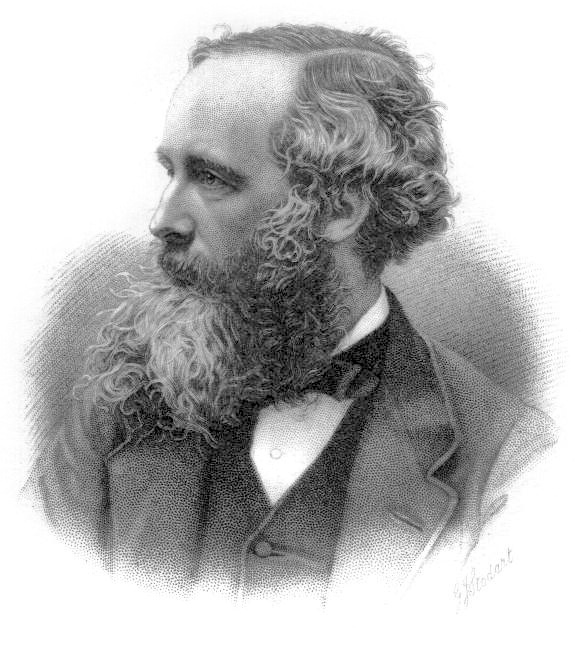
\includegraphics[width=5cm]{images/5.jpg}
	\caption{Nach James Clerk Maxwell sind die bekannten Maxwell-Gleichungen des Elektromagnetismus benannt}
\end{figure}

In der Elektrodynamik werden Phänomene mit bewegten elektrischen Ladungen in Wechselwirkung mit zeitlich veränderlichen elektrischen und magnetischen Feldern beschrieben. Um die Entwicklung der Theorien der Elektrizität und des Magnetismus im 18. und 19. Jahrhundert zusammenzuführen, wurde eine Erweiterung des Theoriengebäudes der klassischen Mechanik notwendig. Ausgangspunkt war das von Michael Faraday entdeckte Induktionsgesetz und die nach Hendrik Antoon Lorentz benannte Lorentzkraft auf eine bewegte elektrische Ladung in einem Magnetfeld. Die Gesetze der Elektrodynamik wurden im 19. Jahrhundert von James Clerk Maxwell zusammengefasst und in Form der Maxwell-Gleichungen erstmals vollständig formuliert. Grundsätzlich wurden elektrodynamische Systeme mit den Methoden der klassischen Mechanik behandelt, allerdings ermöglichen die Maxwell-Gleichungen auch eine Wellenlösung, die elektromagnetische Wellen wie das Licht beschreiben. Diese Theorie brachte unter anderem in Form der Wellenoptik auch einen eigenen Formalismus hervor, der sich grundlegend von dem der klassischen Mechanik unterscheidet. Besonders die Symmetrien der Elektrodynamik sind mit denen der klassischen Mechanik unvereinbar. Dieser Widerspruch zwischen den beiden Theoriegebäuden wurde durch die spezielle Relativitätstheorie gelöst. Die Wellenoptik ist in Form der nichtlinearen Optik noch heute (2011) ein aktives Forschungsgebiet.

\subsection{Thermodynamik}

Etwa gleichzeitig mit der Elektrodynamik entwickelte sich mit der Thermodynamik ein weiterer Theorienkomplex, der sich grundlegend von der klassischen Mechanik unterscheidet. Im Gegensatz zur klassischen Mechanik stehen in der Thermodynamik nicht einzelne Körper im Vordergrund, sondern ein Ensemble aus vielen kleinsten Bausteinen, was zu einem radikal anderen Formalismus führt. Die Thermodynamik eignet sich damit zur Behandlung von Medien aller Aggregatzustände. Die Quantentheorie und die Relativitätstheorie lassen sich in den Formalismus der Thermodynamik einbetten, da sie nur die Dynamik der Bausteine des Ensembles betreffen, aber den Formalismus zur Beschreibung thermodynamischer Systeme nicht prinzipiell ändern.

Die Thermodynamik eignet sich beispielsweise zur Beschreibung von Wärmekraftmaschinen aber auch zur Erklärung vieler moderner Forschungsgegenstände wie Supraleitung oder Suprafluidität. Besonders im Bereich der Festkörperphysik wird daher auch heute (2009) noch viel mit den Methoden der Thermodynamik gearbeitet.

\subsection{Relativitätstheorie}

Die von Albert Einstein begründete Relativitätstheorie führt ein völlig neues Verständnis der Phänomene Raum und Zeit ein. Danach handelt es sich bei diesen nicht um universell gültige Ordnungsstrukturen, sondern räumliche und zeitliche Abstände werden von verschiedenen Beobachtern unterschiedlich beurteilt. Raum und Zeit verschmelzen zu einer vierdimensionalen Raumzeit. Die Gravitation wird auf eine Krümmung dieser Raumzeit zurückgeführt, die durch die Anwesenheit von Masse bzw. Energie hervorgerufen wird. In der Relativitätstheorie wird erstmals die Kosmologie zu einem naturwissenschaftlichen Thema. Die Formulierung der Relativitätstheorie gilt als der Beginn der modernen Physik, auch wenn sie häufig als Vollendung der klassischen Physik bezeichnet wird.

\subsection{Quantenphysik}

Die Quantenphysik beschreibt die Naturgesetze im atomaren und subatomaren Bereich und bricht noch radikaler mit klassischen Vorstellungen als die Relativitätstheorie. In der Quantenphysik sind auch physikalische Größen selbst Teil des Formalismus und keine bloßen Kenngrößen mehr, die ein System beschreiben. Der Formalismus unterscheidet also zwischen zwei Typen von Objekten, den Observablen, die die Größen beschreiben und den Zuständen, die das System beschreiben. Ebenso wird der Messprozess aktiv in die Theorie miteinbezogen. Dies führt in bestimmten Situationen zur Quantisierung der Größenwerte. Das heißt, die Größen nehmen stets nur bestimmte diskrete Werte an. In der Quantenfeldtheorie, der am weitesten entwickelten relativistischen Quantentheorie, tritt auch Materie nur in Portionen, den Elementarteilchen oder Quanten, in Erscheinung.

Die Gesetze der Quantenphysik entziehen sich weitgehend der menschlichen Anschauung, und über ihre Interpretation herrscht auch heute noch kein Konsens. Dennoch zählt sie hinsichtlich ihres empirischen Erfolges zu dem am besten gesicherten Wissen der Menschheit überhaupt.

\section{Themenbereiche der modernen Physik}

Die Theorien der Physik kommen in verschiedenen Themenbereichen zum Einsatz. Die Einteilung der Physik in Unterthemen ist nicht eindeutig und die Abgrenzung der Unterthemen gegeneinander ist dabei ähnlich schwierig wie die Abgrenzung der Physik zu anderen Wissenschaften. Es gibt dementsprechend viele Überschneidungen und gegenseitige Beziehungen der verschiedenen Bereiche zueinander. Hier wird eine Sammlung von Themengebieten nach betrachteter Größenordnung der Objekte dargestellt und im Zuge dessen auf Themengebiete verwiesen, die damit verwandt sind. Die aufgeführten Themen lassen sich nicht eindeutig einer Theorie zuordnen, sondern bedienen sich je nach dem untersuchten Gegenstand verschiedener theoretischer Konzepte.

\subsection{Teilchenphysik}

Die Teilchenphysik befasst sich mit Elementarteilchen und ihren Wechselwirkungen untereinander. Die moderne Physik kennt vier Grundkräfte:
\begin{itemize}
	\item Die Gravitation oder Schwerkraft,
	\item die elektromagnetische Wechselwirkung,
	\item die schwache Wechselwirkung, die beispielsweise für bestimmte radioaktive Zerfallsprozesse verantwortlich ist und
	\item die starke Wechselwirkung, die die Atomkerne zusammenhält.
\end{itemize}
Diese Wechselwirkungen werden durch den Austausch sogenannter Eichbosonen beschrieben. Die Teilchenphysik klammert dabei die Gravitation derzeit (2009) aus, da es noch keine Theorie der Quantengravitation gibt, die die gravitativen Wechselwirkungen von Elementarteilchen vollständig beschreiben kann. In der Teilchenphysik werden relativistische Quantentheorien zur Beschreibung der Phänomene verwendet.

Eines der Ziele der Teilchenphysik ist es, alle Grundkräfte in einem vereinheitlichten Gesamtkonzept zu beschreiben (Weltformel). Bisher ist es jedoch lediglich gelungen, die elektromagnetische Wechselwirkung als Vereinigung der elektrischen und der magnetischen Wechselwirkung darzustellen und ebenso die elektromagnetische Wechselwirkung und die schwache Wechselwirkung zu einer sogenannten elektroschwachen Wechselwirkung zu vereinigen. Zur Vereinigung der elektroschwachen und der starken Wechselwirkung wurde unter anderem die Theorie der Supersymmetrie erdacht, die bislang jedoch nicht experimentell bestätigt werden konnte. Die größten Schwierigkeiten treten wie bereits erwähnt im Bereich der Gravitationskraft auf, da noch keine Theorie der Quantengravitation vorliegt, aber Elementarteilchen nur im Rahmen der Quantentheorie beschrieben werden können.

Typische Experimente zur Überprüfung der Theorien der Teilchenphysik werden an Teilchenbeschleunigern mit hohen Teilchenenergien durchgeführt. Um hohe Kollisionsenergien zu erreichen, werden dabei vor allem Collider-Experimente eingesetzt, bei denen Teilchen gegeneinander und nicht auf ein festes Ziel geschossen werden. Daher wird der Begriff der Hochenergiephysik oft nahezu deckungsgleich mit dem Begriff der Teilchenphysik verwendet. Der Teilchenbeschleuniger mit der derzeit (2011) höchsten Kollisionsenergie ist der Large Hadron Collider. Neutrinodetektoren wie der Super-Kamiokande sind speziell zur Erforschung der Eigenschaften von Neutrinos konzipiert und stellen damit eine zwar spezielle, aber dennoch bedeutende Experimentklasse dar.

\subsection{Hadronen- und Atomkernphysik}

Die Elementarteilchen, die der starken Wechselwirkung unterliegen, die sogenannten Quarks, kommen nicht einzeln, sondern immer nur in gebundenen Zuständen, den Hadronen, vor, zu denen unter anderem das Proton und das Neutron gehören. Die Hadronenphysik hat viele Überschneidungen mit der Elementarteilchenphysik, da viele Phänomene nur erklärt werden können, indem berücksichtigt wird, dass die Hadronen aus Quarks aufgebaut sind. Die Beschreibung der starken Wechselwirkung durch die Quantenchromodynamik, eine relativistische Quantenfeldtheorie, kann jedoch die Eigenschaften der Hadronen nicht vorhersagen, weshalb die Untersuchung dieser Eigenschaften als eigenständiges Forschungsgebiet aufgefasst wird. Es wird also eine Erweiterung der Theorie der starken Wechselwirkung für kleine Energien angestrebt, bei denen sich die Hadronen bilden.

Atomkerne stellen gegenüber Elementarteilchen die nächste Komplexitätsstufe dar. Sie bestehen aus mehreren Nukleonen, also Protonen und Neutronen, deren Wechselwirkungen untersucht werden. In Atomkernen herrschen die starke und die elektromagnetische Wechselwirkung vor. Forschungsgebiete der Atomkernphysik umfassen radioaktive Zerfälle und Stabilität von Atomkernen. Ziel ist dabei die Entwicklung von Kernmodellen, die diese Phänomene erklären können. Dabei wird aber auf eine detaillierte Ausarbeitung der starken Wechselwirkung wie in der Hadronenphysik verzichtet.

Zur Erforschung der Eigenschaften von Hadronen werden Teilchenbeschleuniger eingesetzt, wobei hier der Schwerpunkt nicht so sehr wie in der Teilchenphysik auf hohen Kollisionsenergien liegt. Stattdessen werden Target-Experimente durchgeführt, die zwar geringere Schwerpunktsenergien, aber sehr viel höhere Ereigniszahlen liefern. Allerdings werden auch Collider-Experimente mit Schwerionen vor allem eingesetzt, um Erkenntnisse über Hadronen zu gewinnen. In der Kernphysik werden zur Erzeugung von Transuranen schwere Atome zur Kollision gebracht und Radioaktivität mit einer Vielzahl experimenteller Aufbauten untersucht.

\subsection{Atom- und Molekülphysik}

Atome bestehen aus dem Atomkern und meist mehreren Elektronen und stellen die nächste Komplexitätsstufe der Materie dar. Ziel der Atomphysik ist es unter anderem, die Linienspektren der Atome zu erklären, wozu eine genaue quantenmechanische Beschreibung der Wechselwirkungen der Elektronen der Atome notwendig ist. Da Moleküle aus mehreren Atomen aufgebaut sind, arbeitet die Molekülphysik mit ähnlichen Methoden, allerdings stellen insbesondere große Moleküle meist deutlich komplexere Systeme dar, was die Rechnungen sehr viel komplizierter und häufig den Einsatz von Computersimulationen erforderlich macht.

Die Atom- und Molekülphysik stehen über die Untersuchung der optischen Spektren von Atomen und Molekülen mit der Optik in enger Beziehung. So baut beispielsweise das Funktionsprinzip des Lasers, einer bedeutenden technischen Entwicklung, maßgeblich auf den Ergebnissen der Atomphysik auf. Da die Molekülphysik sich auch intensiv mit der Theorie der chemischen Bindungen befasst, sind in diesem Themengebiet Überschneidungen mit der Chemie vorhanden.

Ein wichtiger experimenteller Zugang besteht in der Einwirkung von Licht. So werden beispielsweise optische Spektren von Atomen und Molekülen mit ihren quantenmechanischen Eigenschaften in Verbindung gesetzt. Umgekehrt kann dann mit spektroskopischen Methoden die Zusammensetzung eines Stoffgemisches untersucht werden und anhand von Sternenlicht Aussagen über die Elemente in der Sternenatmosphäre getroffen werden. Andere Untersuchungsmethoden betrachten das Verhalten unter dem Einfluss von elektrischen und magnetischen Feldern. Beispiele sind die Massenspektroskopie oder die Paulfalle.

\subsection{Kondensierte Materie und Fluiddynamik}

Die Physik der kondensierten Materie und die Fluiddynamik sind in dieser Auflistung das Gebiet mit der größten thematischen Bandbreite, von der Festkörperphysik bis zur Plasmaphysik. All diesen Bereichen ist gemeinsam, dass sie sich mit makroskopischen Systemen aus sehr vielen Atomen, Molekülen oder Ionen befassen. Dementsprechend ist in allen Bereichen dieses Themengebiets die Thermodynamik ein wichtiger Teil des theoretischen Fundamentes. Je nach Problem kommen aber auch Quantentheorie und Relativitätstheorie zum Einsatz, um die Systeme zu beschreiben. Auch Computersimulationen sind ein fester Bestand der Forschung an solchen Vielteilchensystemen.

Aufgrund der thematischen Bandbreite existieren Überschneidungen mit nahezu allen anderen Gebieten der Physik, zum Beispiel mit der Optik in Form laseraktiver Medien oder nichtlinearer Optik, aber auch mit der Akustik, Atom-, Kern- und Teilchenphysik. Auch in der Astrophysik spielt die Fluiddynamik eine große Rolle bei der Erstellung von Modellen zur Entstehung und zum Aufbau von Sternen sowie bei der Modellierung vieler anderer Effekte. Viele Forschungsbereiche sind dabei sehr anwendungsorientiert, wie die Materialforschung, die Plasmaphysik oder die Erforschung der Hochtemperatursupraleiter.

Die Bandbreite der experimentellen Methoden in diesem Bereich der Physik ist sehr groß, sodass sich keine typischen Methoden für das ganze Gebiet angeben lassen. Die quantenmechanischen Effekte wie Supraleitung und Suprafluidität, die eine gewisse Bekanntheit erlangt haben, werden der Tieftemperaturphysik zugerechnet, die mit typischen Kühlungsmethoden einhergeht.

\subsection{Astrophysik und Kosmologie}

Astrophysik und Kosmologie sind interdisziplinäre Forschungsgebiete, die sich stark mit der Astronomie überschneiden. Nahezu alle anderen Themenbereiche der Physik gehen in die astrophysikalischen Modelle ein, um Prozesse auf verschiedenen Größenskalen zu modellieren. Ziel dieser Modelle ist es, astronomische Beobachtungen auf der Grundlage der bisher bekannten Physik zu erklären.

Die Kosmologie baut insbesondere auf den Grundlagen der allgemeinen Relativitätstheorie auf, allerdings sind im Rahmen der Quantenkosmologie auch die Quantentheorien sehr bedeutsam um die Entwicklung des Universums in sehr viel früheren Phasen zu erklären. Das derzeit (2009) am meisten vertretene kosmologische Standardmodell baut dabei maßgeblich auf den Theorien der Dunklen Materie und der Dunklen Energie auf. Weder Dunkle Materie noch Dunkle Energie konnte bisher direkt experimentell nachgewiesen werden, es existieren aber eine Vielzahl von Theorien, was genau diese Objekte sind.

Da in der Astrophysik nur in sehr beschränktem Ausmaß Experimente möglich sind, ist dieses Teilgebiet der Physik sehr stark auf die Beobachtung unbeeinflussbarer Phänomene angewiesen. Dabei kommen auch Erkenntnisse der Atomphysik und der Teilchenphysik und typische Messmethoden dieser Fachgebiete zur Anwendung, um Rückschlüsse auf astrophysikalische oder kosmologische Zusammenhänge zu ziehen. Beispielsweise geben die Spektren von Sternenlicht Auskunft über die Elementverteilung der Sternenatmosphäre, die Untersuchung der Höhenstrahlung erlaubt Rückschlüsse auf die kosmische Strahlung und Neutrinodetektoren messen nach einer Supernova einen erhöhten Neutrinostrom, der gleichzeitig mit dem Licht der Supernova beobachtet wird.

\subsection{Interdisziplinäre Themenbereiche}

Methoden der Physik finden in vielen Themengebieten Anwendung, die nicht zum Kern\-themen\-bereich der Physik gehören. Einige dieser Anwendungen sind in den vorigen Kapiteln bereits angesprochen worden. Die folgende Aufzählung gibt einen kurzen Überblick über die wichtigsten interdisziplinären Themenbereiche.
\begin{itemize}
	\item Die Astrophysik wendet physikalische Methoden auf das Studium astronomischer Phänomene an.
	\item In der Biophysik werden die physikalischen Gesetzmäßigkeiten untersucht, denen Lebewesen und ihre Wechselwirkung mit der Natur unterliegen.
	\item Die Medizinische Physik nutzt physikalische Phänomene wie zum Beispiel Laser, Radioaktivität, Röntgenstrahlung und Kernspinresonanz für medizinische Diagnostik und Therapie.
	\item Bei der physikalischen Chemie werden Methoden der Physik auf die Anschauungsobjekte der Chemie angewendet.
	\item Die Geophysik nutzt physikalische Modelle und Methoden zur Erklärung geowissenschaftlicher Vorgänge und Fragestellungen.
	\item Die Technische Physik befasst sich mit den technischen Anwendungen physikalischen Wissens. Wichtige Teilbereiche sind die Quantenelektronik und die Theorie der Quantencomputer.
	\item Die Umweltphysik beschäftigt sich in ihrer Forschung vor allem mit den Bereichen Energie und Klima.
	\item Soziophysik und Ökonophysik wenden physikalische und statistische Methoden auf gesellschaftliche, wirtschaftliche, kulturelle und politische Phänomene an.
\end{itemize}

\section{Grenzen der physikalischen Erkenntnis}

Der derzeitige Stand der Physik ist nach wie vor mit noch ungelösten Problemen konfrontiert. Zum einen handelt es sich dabei um den weniger grundsätzlichen Fall von Problemen, deren Lösung prinzipiell möglich, aber mit den derzeitigen mathematischen Möglichkeiten bestenfalls annäherbar ist. Zum anderen gibt es eine Reihe von Problemen, für die noch unklar ist, ob eine Lösung im Begriffsrahmen der heutigen Theorien überhaupt möglich sein wird. So ist es bislang nicht gelungen, eine vereinheitlichte Theorie zu formulieren, welche sowohl Phänomene beschreibt, die der elektroschwachen wie der starken Wechselwirkung unterliegen, wie auch solche, welche der Gravitation unterliegen. Erst bei einer solchen Vereinigung von Quantentheorie und Gravitationstheorie (allgemeiner Relativitätstheorie) könnten alle vier Grundkräfte einheitlich behandelt werden, sodass eine vereinheitlichte Theorie der Elementarteilchen resultierte.

Die bisherigen Kandidaten von Quantengravitationstheorien, Supersymmetrie und Supergravitations-, String- und M-Theorien versuchen, eine solche Vereinheitlichung zu erreichen. Überhaupt ist es ein praktisch leitendes Ziel heutiger Physiker, sämtliche Vorgänge der Natur durch eine möglichst geringe Anzahl von möglichst einfachen Naturgesetzen zu beschreiben. Diese sollen das Verhalten möglichst grundlegender Eigenschaften und Objekte (etwa Elementarteilchen) beschreiben, sodass höherstufige (emergente) Prozesse und Objekte auf diese Beschreibungsebene reduzierbar sind.

Ob dieses Ziel prinzipiell oder praktisch erreichbar ist, ist eigentlich nicht mehr Gegenstand der einzelwissenschaftlichen physikalischen Erkenntnisbemühung, ebenso wenig, wie es allgemeine Fragen darüber sind, welchen Gewissheitsgrad physikalische Erkenntnisse grundsätzlich erreichen können oder faktisch erreicht haben. Derartige Fragen sind Gegenstand der Epistemologie und Wissenschaftstheorie. Dabei werden ganz unterschiedliche Positionen verteidigt. Relativ unbestritten ist, dass naturwissenschaftliche Theoriebildungen in dem Sinne nur Hypothesen sind, dass man nicht mit Gewissheit wissen kann, ob es sich dabei um wahre und gerechtfertigte Auffassungen handelt. Man kann hier noch in spezifischerer Weise vorsichtig sein, indem man sich auf die Theorie- und Begriffsvermitteltheit aller empirischen Erkenntnisse beruft oder auf die Tatsache, dass der Mensch als erkennendes Subjekt ja unter den Gegenstandsbereich physikalischer Theorien fällt, aber nur als wirklich Außenstehender sicheres Wissen haben könnte. Denn für Beobachter, die mit ihrem Erkenntnisobjekt interagieren, bestehen prinzipielle Grenzen der Prognostizierbarkeit im Sinne einer Ununterscheidbarkeit des vorliegenden Zustandes -- eine Grenze, die auch dann gelten würde,\footnote{Vgl. Esfeld, Naturphilosophie, 128.} wenn der Mensch alle Naturgesetze kennen würde und die Welt deterministisch wäre. Diese Grenze hat praktische Bedeutung bei deterministischen Prozessen, für welche geringe Änderungen des Anfangszustands zu großen Abweichungen in Folgezuständen führen -- Prozesse, wie sie durch die Chaostheorie beschrieben werden. Aber nicht nur eine praktische Voraussagbarkeit ist in vielen Fällen nur begrenzt möglich, auch wird von einigen Wissenschaftstheoretikern eine Aussagefähigkeit physikalischer Modelle über die Realität überhaupt bestritten. Dies gilt in verschiedenen Ausarbeitungen eines sogenannten wissenschaftstheoretischen Antirealismus in unterschiedlichem Ausmaß: für unterschiedliche Typen physikalischer Begriffe wird eine reale Referenz bestritten oder für unwissbar gehalten.\footnote{Vgl. Eintrag in Edward N. Zalta (Hrsg.): \emph{Stanford Encyclopedia of Philosophy.}} Auch eine prinzipielle oder wahrscheinliche Zusammenführbarkeit einzelner Theorien wird von einigen Wissenschaftstheoretikern bestritten.\footnote{Vgl. \emph{Scientific Progress.} In: Edward N. Zalta (Hrsg.): \emph{Stanford Encyclopedia of Philosophy.} und \emph{The Unity of Science.} In: Edward N. Zalta (Hrsg.): \emph{Stanford Encyclopedia of Philosophy.}; Esfeld, Naturphilosophie, S.\,100--115.}

\section{Beziehung zu anderen Wissenschaften}

Die Beziehungen zur Philosophie sind traditionell eng, hat sich doch die Physik aus der klassischen Philosophie entwickelt, ohne ihr jemals grundsätzlich zu widersprechen, und waren nach heutigen Kategorien zahlreiche bedeutende Physiker zugleich wichtige Philosophen und umgekehrt. Gemäß der heutigen philosophischen Disziplinenunterscheidung ist die Physik insbesondere auf die Ontologie bezogen, welche die Grundstrukturen der Realität in möglichst allgemeinen Begriffen zu beschreiben versucht, darüber hinaus auf die Erkenntnistheorie, welche die Gütekriterien von Wissen überhaupt zu erfassen versucht, spezieller noch auf die Wissenschaftstheorie, welche die allgemeinen Methoden wissenschaftlicher Erkenntnis zu bestimmen versucht und natürlich auf die Naturphilosophie bzw. Philosophie der Physik, die oftmals als Unterdisziplin der Ontologie oder Wissenschaftstheorie behandelt wird, jedenfalls aber spezieller gerade auf die Einzelerkenntnisse der Physik bezogen arbeitet, deren Begriffssystem analysiert und ontologische Interpretationen physikalischer Theorien diskutiert.

\section{Physik in der Gesellschaft}

\begin{figure}
	\centering
	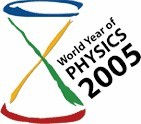
\includegraphics[width=4cm]{images/6.jpg}
	\caption{Logo des Jahres der Physik 2005}
\end{figure}

Da die Physik als die grundlegende Naturwissenschaft gilt, werden physikalisches Wissen und Denken bereits in der Schule meist im Rahmen eines eigenen Schulfaches unterrichtet. Im Rahmen des Schulsystems wird Physik in der Regel als Nebenfach ab Klassenstufe 5--7 unterrichtet, und wird in der Oberstufe oft auch als Leistungskurs geführt.
\begin{itemize}
	\item Die meisten Universitäten bieten das Studienfach Physik an.
	\item Seit 1901 vergibt die Schwedische Akademie der Wissenschaften jährlich den Nobelpreis für Physik.
	\item Die Frage nach der Ethik naturwissenschaftlicher Forschung wurde erstmals explizit aufgeworfen, als physikalische Entdeckungen Ende der 1930er Jahre auf die Möglichkeit einer Atombombe hindeuteten. Dieses Thema wird auch in der Literatur, etwa in Friedrich Dürrenmatts Theaterstück \emph{Die Physiker} aufgegriffen.
	\item 2005 war das Jahr der Physik.
\end{itemize}

\begin{thebibliography}{7}
	\bibitem{Ber} Ludwig Bergmann, Clemens Schaefer, Thomas Dorfmüller, Wilhelm T. Hering, Klaus Stierstadt: \emph{Lehrbuch der Experimentalphysik.} 11. Auflage, de Gruyter, 1998, ISBN 3-11-012870-5
	\bibitem{Dem} Wolfgang Demtröder: \emph{Experimentalphysik.} 4. Auflage, Springer, 2005, ISBN 3-540-26034-X
	\bibitem{Lan} Lew Dawidowitsch Landau, Jewgeni Michailowitsch Lifschitz: \emph{Lehrbuch der theoretischen Physik} in 10 Bänden, Akademie-Verlag Berlin, neu: Harri Deutsch-Verlag Frankfurt/Main
	\bibitem{Fey} Richard Feynman, Robert Leighton, Matthew Sands: \emph{Feynman-Vorlesungen über Physik} Oldenbourg, 1999, ISBN 3-486-25857-5
	\bibitem{Ger} Christian Gerthsen, Dieter Meschede: \emph{Gerthsen Physik.} 23.~Auflage. Springer-Verlag, 2006, ISBN 3-540-25421-8
	\bibitem{Sei} Walter Seitter: \emph{Physik des Daseins. Bausteine zu einer Philosophie der Erscheinungen}. Sonderzahl, Wien 1997, ISBN 3-85449-120-4
	\bibitem{Tip} Paul A. Tipler, Gene Mosca: \emph{Physik für Wissenschaftler und Ingenieure.} 2. Auflage, Elsevier Spektrum Akademischer Verlag, München/Heidelberg 2004, ISBN 3-8274-1164-5.
\end{thebibliography}

\end{document}

